In physics there exist mathematical structures known as topological defects that are singularities that cannot be removed without affecting the system at large scales.
Condensed matter systems provide many examples of the existence of topological defects. A particular case are vortex-like structures: at low temperatures, there are magnetic flux lines in type II superconductors and quantized vortex lines in superfluid $^{3}$He and $^4$He \cite{Zurek1985,Zurek1993,Zurek1996,bunkov,PhysRevLett.43.214,ancio2015}.

\section{Topological defects}\label{sec:topdef}
In order to define a topological defect, we first review some other definitions. Generally speaking, an \textit{order parameter} can be any quantity that is defined in a physical system, in space or spacetime, that distinguishes between ordered and disordered phases. It is zero when the system is in the disordered phase, and non-zero when it is in the ordered phase. The set of values that the order parameter can take is called the \textit{order parameter space} or \textit{order parameter manifold}.

A topological defect can be defined as a discontinuity in the order pa\-ram\-e\-ter space of a system. The definition suggests that an order parameter is related to changes of phases, spontaneous symmetry breaking, etc. Top\-o\-log\-i\-cal defects have the feature that they are extremely stable, meaning that no local rearrangement of the order parameter can remove them. 

The study of topological defects rely on homotopy theory. Homotopy theory deals with the use of continuous deformations that transform one object into another thus establishing their topological equivalence. A par\-tic\-u\-lar\-ly simple deformable object is a \textit{path} and if the path is closed it is called a \textit{loop}. In the following we give some useful definitions in topology. Sections \ref{sec:topdef} and  \ref{sec:examples} are based on Ref.\ \cite{mermin1979}. 

%Examples of ordered media are the spin models. An 'spin' is defined as a vector quantity of $n$ dimensions attached to every point a given region, usually spins are normalize to unity.


\subsection{Review of topology}\label{sec:revtop}
The study of topology in physics is important. In particular, the topology of the vacuum manifold $\mathcal{M}$ defines what topological defect can arise. %More specifically, the behavior of topological defects is studied by homotopy theory.

 
%\begin{definition}
%Two continuous maps between topological spaces $f: X\to Y$ and $g: X\to Y$ are \textbf{homotopic} if there exists a continuous function
%\begin{equation}
%	H: X\times[0,1]\to Y,
%\end{equation}
%such that
%\begin{equation}
%	H(x,0) = f(x), \ \ \ H(x,1) = g(x).
%\end{equation}
%\end{definition}
\begin{definition}[Topology]
Let the set $X\neq \emptyset$. A collection of subsets $\tau$ of $X$, called open sets, is said to be a \textit{topology} if they satisfy the following properties:
\begin{enumerate}
\item $X,\emptyset \in \tau$,
\item $U_1,\ U_2 \in \tau \Rightarrow U_1\cap U_2 \in \tau$,
\item $U_i \in \tau$, $\forall i\in I\Rightarrow$ $\bigcup_{i\in I} U_i \in \tau$, where $I$ is a set of indices.
\end{enumerate}
The pair $(X,\tau)$ is called a \textit{topological space}.
\end{definition}
The appeal of a topological space is that it is the most general space one can work with, in the sense that closeness can be defined by the definition above. The definition of path connectedness and the idea of loops can be used to describe the holes in a topological space.

\begin{definition}[Path]
Let $x_0,x_1\in X$. A \textit{path} $\gamma$ in $X$ from $x_0$ to $x_1$ is a continuous map
\begin{equation}
	\gamma: [0,1] \to X,
\end{equation}
with
\begin{equation}
	\gamma(0) = x_0, \ \ \ \gamma(1) = x_1.
\end{equation}
\end{definition}
We say that a topological space $X$ is \textit{path connected} if there exists a path connecting any two points $x_0,x_1\in X$.

\begin{definition}[Loop]
 A \textit{loop} in a topological space $X$ at the base point $x_0 \in X$ is a continuous map 
 \begin{equation}
	\gamma: [0,1] \to X,
\end{equation}
with
 \begin{equation}
 	\gamma(0) = \gamma(1) = x_0.
 \end{equation}
 Equivalently we can write  this map as
 \begin{equation}
 	\gamma : S^1 \to X,
 \end{equation}
 where $S^1$ is the 1-sphere.
 The space of all loops at $x_0\in X$ or \textit{loop space} at the base point $x_0\in X$ is denoted $\mathscr{C}_{x_0}(X)$.
\end{definition}
The loops defined above are also called 1-dimensional loops and can be generalized to higher dimensions. An $n$-th loop is a smooth map from the $n$-sphere to the topological space $\gamma : S^{n} \to X$.
\begin{definition}[Constant loop] The \textit{constant loop} $e$ at $x_0\in X$ is defined as
	\begin{equation}
		e(t) = x_0, \ \ \ 0\leq t \leq 1.
	\end{equation}
\end{definition}

\begin{definition}[Inverse loop]
Consider the loop $\gamma$ at $x_0\in X$. Its \textit{inverse loop} $\gamma^{-1}$ is defined as 
	\begin{equation}
		\gamma^{-1}(t) = \gamma(1-t), \ \ \ 0 \leq t \leq 1.
	\end{equation}
\end{definition}

\begin{definition}[Homotopic loops] Two loops $\gamma$ and $\gamma'$ at $x_0 \in X$ are \textit{homotopic loops} denoted $\gamma \sim \gamma'$, if there exists a continuous map
\begin{equation}
	H: [0,1]\times[0,1] \to X,
\end{equation}
such that
\begin{eqnarray}
	H(t,0) = \gamma(t), & & 0\leq t \leq 1, \nonumber \\ 
	H(t,1) = \gamma'(t), & & 0\leq t \leq 1,  \nonumber\\
	H(0,s) = H(1,s) = x_0, & & 0\leq s \leq 1. 
\end{eqnarray}
\end{definition}

The homotopy of loops, and more generally of paths, forms an equivalence relation meaning that they satisfy the properties of \textit{symmetry}, \textit{reflexivity} and \textit{transitivity}. %Clearly, a loop $\gamma$ is homotopic to itself, satisfying reflexivity, that is $\gamma\sim\gamma$
Reflexivity means that an element $a$ of an equivalence relation is equivalent to itself, that is, $a\sim a$. If $a$ and $b$ are elements of the equivalence relation, symmetry implies $a\sim b$ if and only if $b\sim a$. Transitivity means that that if $a\sim b$ and $b\sim c$ then $a\sim c$.


We denote an equivalence class as $[\gamma] = \{\gamma' | \gamma' \sim \gamma \}$. One important feature of loops is that we can define a product between them by consecutively following one after the other.
\begin{definition}[Product of loops] The \textit{product of loops}
\begin{equation}
	\star: \mathscr{C}_{x_0}(X)\otimes \mathscr{C}_{x_0}(X) \to \mathscr{C}_{x_0}(X).
\end{equation}
For any two loops at $x_0\in X$, $\gamma, \gamma' \in \mathscr{C}_{x_0}(X)$, the \textit{product loop} $\rho = \gamma \star \gamma' \in \mathscr{C}_{x_0}(X)$ is given by
\begin{equation}
	\rho(t) = (\gamma \star \gamma') (t)= \begin{cases} 
              	\gamma(2t), & 0\leq t \leq 1/2,\\
              	\gamma'(2t-1),&  1/2 < t \leq 1.
	          \end{cases}
\end{equation}
\end{definition}
%The homotopy class of loops forms a group under the operation of the product of loops.
The most important feature of loops is that their set of homotopy classes at a point $x_0\in X$ forms a group under the product of loops, where the identity is $I=[e]$ and the inverse is $[\gamma]^{-1}=[\gamma^{-1}]$. This group is called the \textit{first homotopy group} or \textit{fundamental group}, and it is denoted as $\pi_1(X,x_0)$. If the space $X$ is path connected, we can ignore the base point $x_0\in X$ because it can be shown that the first homotopy groups of $X$ at any two point $x_0,x_1\in X$ are isomorphic $\pi_1(X,x_0)\simeq \pi_1(X,x_1)$. We then write $\pi_1(X)$ to refer to the first homotopy group.
%Before proceeding with higher homotopy groups we discuss briefly some important concepts in group theory.

\subsection{Higher homotopy groups}\label{sec:homgroup}
We can define the $n$-th homotopy group of $X$ denoted $\pi_n(X)$, where $n$ is the dimension of the loop. In particular, if we take the topological space $X$ to be an $i$-sphere, then the $n$-th homotopy group summarizes all the possible ways a $n$-sphere wraps around a $i$-sphere.

For example, the first homotopy group of a 1-sphere, $\pi_1(S^1)$, contains information on how a circle can be mapped onto another circle. It can be wrapped once, or several times, be wrapped in the opposite direction, or not be wrapped at all. This defines the first homotopy group of the 1-sphere to be isomorphic to the set of integers $\mathbb{Z}$, so we write $\pi_1(S^1) \simeq \mathbb{Z}$. In general, $\pi_n(S^n) \simeq \mathbb{Z}$, in this case we define the \textit{winding number} or \textit{topological charge} $m\in \mathbb{Z}$, which is the number of times a $n$-loop is wrapped around a $n$-sphere. We can use the winding number to classify different configurations that fall into the same equivalence class. Two configurations are topologically equivalent if they have the same winding number.

If the homotopy group of the order parameter manifold $\mathcal{M}$ is non-trivial, it enables topological defects. In particular, if the first homotopy group is non-trivial, then vortex-like solutions appear. If the vortex-like solution appears in 3 spatial dimensions, it is called a \textit{string}. We list some topological defects defined by the non-triviality of the homotopy group of the order parameter manifold:

\begin{itemize}
\item $\pi_0(\mathcal{M}) \neq I$ $\to$ \textit{Kinks or  Domain Walls}
\item $\pi_1(\mathcal{M}) \neq I$ $\to$ \textit{Vortex/Strings}
\item $\pi_2(\mathcal{M}) \neq I$ $\to$ \textit{Monopoles}
\item $\pi_3(\mathcal{M}) \neq I$ $\to$ \textit{Textures or Instantons}
\end{itemize}

In practice it is useful to describe the order parameter space/manifold as a \textit{coset space/manifold}. Before proceeding along these lines, we review some useful concepts in group theory.

\subsection{Review of group theory}\label{sec:revgroup}
In physics, symmetry is vital. In particular, gauge theories are based on local symmetries. For example, electroweak theory, quantum chromodynamics, and general relativity are all gauge theories. A symmetry refers to an in\-va\-ri\-ance of a quantity (the Lagrangian, Hamiltonian, etc.) under a group of trans\-for\-ma\-tions. We review some basic concepts and definitions of group theory, following Refs.\ \cite{Nakahara2003,Malek2018}.
\begin{definition}[Group]
A set of elements $G$ is a \textit{group} under some operation $``\cdot": G\times G \to G$, often called the \textit{product}, if it satisfies the following:
\begin{enumerate}
\item \textbf{Closure}: If $\forall\, g_1, g_2 \in G$, then also $g_1 \cdot g_2 \in G$.
\item \textbf{Associativity}: If $\forall\, g_1, g_2, g_3 \in G$ then it must be true that $(g_1\cdot g_2)\cdot g_3 = g_1\cdot (g_2\cdot g_3)$.
\item \textbf{Identity}: $\exists \, e \in G$ such that $\forall g \in G$, $e\cdot g = g \cdot e = g$.
\item \textbf{Inverse}: $\forall g \in G$, $\exists \,g^{-1} \in G$ such that $g^{-1}\cdot g = g \cdot g^{-1} = e$.
\end{enumerate}
\end{definition}
%We usually leave out the product symbol $\cdot$ and write $g_1g_2$. 

\begin{definition}[Subgroup]
If $G$ is a group and $H$ is a subset of $G$, denoted $H\subset G$, such that the elements of $H$ form a group, then we say that $H$ forms a \textit{subgroup }of $G$.
\end{definition}

Examples of groups are:
\begin{itemize}
 \item The orthogonal group O$(n)$ can be represented by the set of all $n\times n$ real matrices that preserve the inner product in $\mathbb{R}^n$.
\item The special orthogonal groups SO$(n)$ can be represented by the subgroup of matrices in O$(n)$ that have determinant 1.
\item The unitary group U$(n)$ can be represented by the set of $n\times n$ complex matrices that preserve the inner product in $\mathbb{C}^n$.
\item The special unitary group SU$(n)$ can be represented by the subgroup of matrices in U$(n)$ that have determinant $1$. 
\end{itemize} 
The groups listed above are submanifolds of their corresponding vector spaces of $n\times n$ matrices. These kinds of groups are called \textit{Lie groups}.
\begin{definition}[Lie group]
A \textit{Lie group} is a group which is also a smooth manifold.
\end{definition} 

The importance of a Lie group is that it is continuous, so that we can study it with the tools of differential geometry.

\begin{definition}[Homomorphism] Given two groups $G$ and $H$, we say that $\rho: G \to H$ is an \textit{homomorphism} if
\begin{equation}
	\rho(g\cdot h) = \rho(g)\rho(h),
\end{equation}
where $g\in G$ and $h\in H$.
\end{definition}

\begin{definition}[Representation of a group]
Given a group $G$ with elements $g_1, g_2, \dots$, we call $D(g_i)$ the \textit{representation of the group} which is a homomorphism from the group $G$ to the group of $n\times n$ matrices so that the elements of $G$ are $D(e), \, D(g_1),\dots$. Each $D(g_i)$ is a matrix of dimension $n$. We can then choose the product ``$\cdot$" to be the matrix multiplication, such that, $D(g_i)\cdot D(g_j) = D(g_i\cdot g_j)$.
\end{definition}
\begin{definition}[Left and right cosets]
Let $G$ be a group and $H\subset G$ a subgroup of $G$ and $g\in G$, then $\forall g \in G$
 \begin{itemize}
 \item The set $gH = \{g\cdot h| h\in H\}$ is called the \textit{left coset} of $H$ in $G$.
 \item The set $Hg = \{h\cdot g| h\in H\}$ is called the \textit{right coset} of $H$ in $G$.
 \end{itemize}
\end{definition}

\begin{definition}[Normal subgroup]
$H$ is a \textit{normal subgroup} of $G$ if $gH = Hg$, that is, if the left and right cosets are equal.
\end{definition}

\begin{definition}[Quotient group]
If $G$ is a group and $H\subset G$ is normal, then we define the \textit{factor group} or \textit{quotient group} or \textit{coset group}, denoted as $G/H$ (read ``$G$ modulo $H$"), as the group with elements in the set
\begin{equation}
	G/H \equiv \{gH|g\in G\},
\end{equation} 
that is, the set of all left cosets of $H$ in $G$.
\end{definition}
%{\tt One way of thinking about a quotient group is that it is the set of elements of $G$ that are not in $H$. All the subsets in $G$ related by operations in $H$ are considered as identical.}
In practice we often call the left coset just the coset group. 

It is important to note that we can form equivalence classes in the group $G$ related by operations in $H$. We say that $g_1, g_2\in G$ are equivalent if there exists an element in $h\in H$ such that $g_1 = g_2 \cdot h$. Two elements in $G$ are said to be in the same equivalence class if they are equivalent. We can then define the space or manifold by associating each equivalence class with a point. The resulting manifold is known as the \textit{coset space} or \textit{coset manifold} $G/H$.

%A more practical way of thinking about the \textit{coset} group is that it is the set of elements in $G$ that are related by operations in $H$, that is, the set of elements of $G$ 
As an illustration, we study the coset space SO$(3)/$SO$(2)$ and see that it is isomorphic to the manifold $S^2$. We take a point $P$ in the 2-sphere $S^2$ and call $\hat{u}$ the unit vector pointing to $P$. Let $\hat{z}$ be the unit vector pointing to $(0,0,1)$. Let $g_1\in $ SO$(3)$  such that $\hat{z}=g_1\hat{u}$. We could associate $g_1$ to $P$ in order to form the manifold. However, the transformation that takes $\hat{u}$ to $\hat{z}$ is not unique. We call $h\in $ SO$(2)$ a rotation about the $z$-axis, and we relate two transformations $g_1$ and $g_2$ in SO$(3)$ if $g_1 = g_2 h$, that is, if both take $\hat{u}$ to $\hat{z}$. Therefore, we need to remove the redundant transformations. So, we do not associate $g_1$ to the point $P$ but all the equivalence classes of $g_1$, that is, we associate $P$ to an element of the group SO$(3)/$SO$(2)$. In other words, the manifold associated to SO$(3)/$SO$(2)$ is indeed $S^2$.

\subsection{Order parameter spaces as coset spaces}\label{sec:orderparam}
As we discussed, the order parameter manifold is related to a reduction of symmetry.  
For example, in an ordered medium, we only need to find the fundamental representation of the group of symmetries of the physical space, say $G$, and find the group of isometries $H$ of the system, then the parameter space is $G/H$. As an example, we take a vector field in the 3-dimensional space with constant length as our order parameter. The physical space has an SO$(3)$ symmetry, and the vector field is invariant under SO$(2)$ rotations along its axis, therefore, the order parameter space is  SO$(3)/$SO$(2) \simeq S^2$ (as we saw earlier). 

In field theory, if we want to describe the order parameter manifold of a field after Spontaneous Symmetry Breaking (SSB), we first consider the symmetry group $G$ before SSB and then the symmetry group $H$ after SSB. Then, the order parameter space is $G/H$ (as we will see in Section \ref{sec:qft}). 

\section{Examples of topological defects in physics}\label{sec:examples}

\subsection{The planar spin model in 2-dimensions}\label{sec:XY}
Let us illustrate the idea of a topological defect with the XY model in two dimensions. In this case, we take the order parameter as a vector quantity called the classical spin $\vec{s}\in \mathbb{R}^2$
\begin{equation}
	\vec{s}(\vec{r}\,) = \begin{pmatrix}
	\cos\varphi \\
	\sin\varphi
\end{pmatrix},\ \varphi \equiv \varphi(\vec{r}),\ |\vec{s}\,| = 1, \  \vec{r}\in\mathbb{R}^2.
\end{equation}
Physically, if the system that we study using this model is a ferromagnet, we call the spin $\vec{s}$ the local magnetization.

Suppose $\vec{s}$ to be a continuous function of $\vec{r}$ except at a point $P$ in the plane, and that we know $\vec{s}$ on a circle of radius $R$ around the point $P$. We consider all the field vectors $\vec{s}$ that lie along the circle.  Since the field is continuous on the circle, the angle $\varphi$ of the vector field $\vec{s}$ as we travel along the circle will be an integer multiple of $2\pi$, that is $2\pi n$, where $n\in\mathbb{Z}$ is the \textit{winding number} or \textit{topological charge}. This way we can classify different singular configurations that fall into the same equivalence class given their winding numbers.

The spins create an \textit{order parameter space} or \textit{order parameter manifold} which is the space formed by all the possible values of the order parameter. In this case, the spins in two dimensions can take values along the circumference of radius 1, therefore, the order parameter space is $S^1/I \simeq S^1$. The spin angle $\varphi$ in the plane can be mapped to the spin space and it is represented as a point in the order parameter manifold. Generally speaking, the specification of the order parameter along a curve in real space, as opposed to spin space, determines a mapping of that curve in the order parameter manifold. If the curve in real space is closed, the mapping also determines a closed curve in the order parameter space. The number of times that the mapping wraps around the closed curve in the order parameter space is the winding number.  

It is easy to see that the only topological defects are \textit{vortices}, since $\pi_1(S^1) \simeq \mathbb{Z}$ and $\pi_m(S^1) \simeq I$, $m > 1$.

%We say that two different field configurations are \textit{topological equivalent}, since we can continuously deformed one into the other without altering the winding number in a region far away from the singular point. %Configurations with the same winding number fall in the same equivalence class.


 In Figure \ref{fig:vortices} we see different spin configurations with several winding numbers $n$.
\begin{figure}
	\centering
	\begin{subfigure}{0.45\textwidth}
		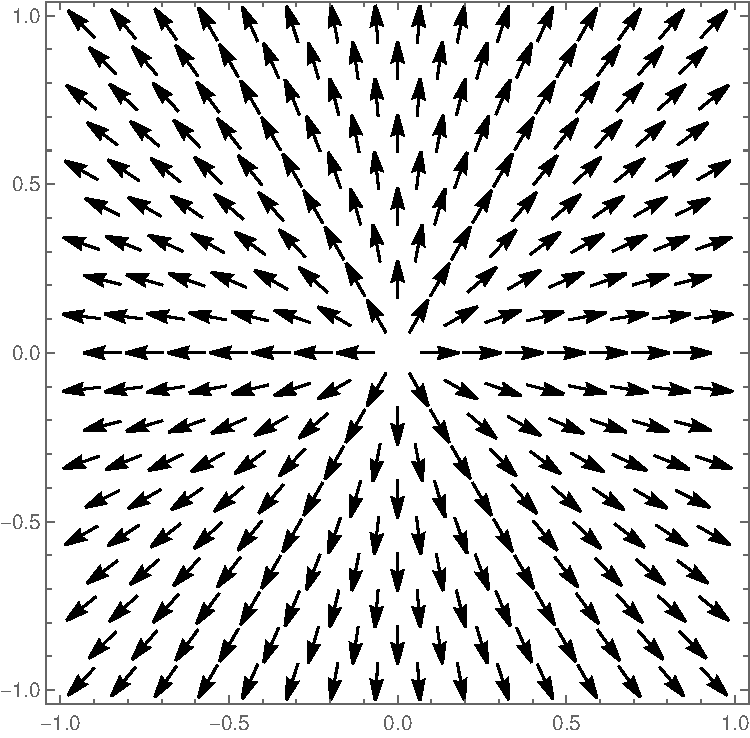
\includegraphics[scale=1,trim= 120 100 100 100,clip]{./figures/vortex.pdf}
		\caption{$n=1$}
	\end{subfigure}
	\begin{subfigure}{0.45\textwidth}
		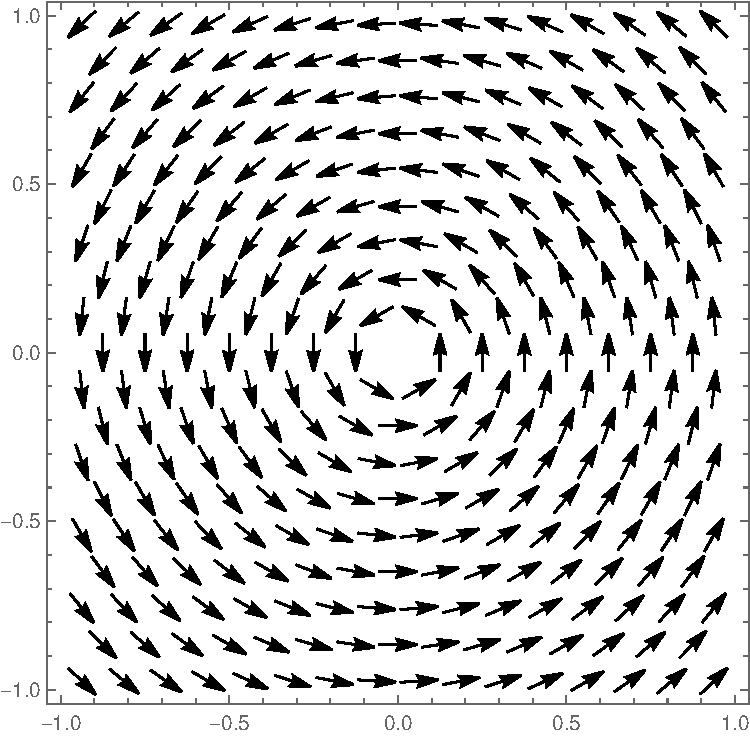
\includegraphics[scale=1,trim= 120 100 100 100,clip]{./figures/vortex2.pdf}
		\caption{$n=1$}
	\end{subfigure}
	
	\begin{subfigure}{0.45\textwidth}
		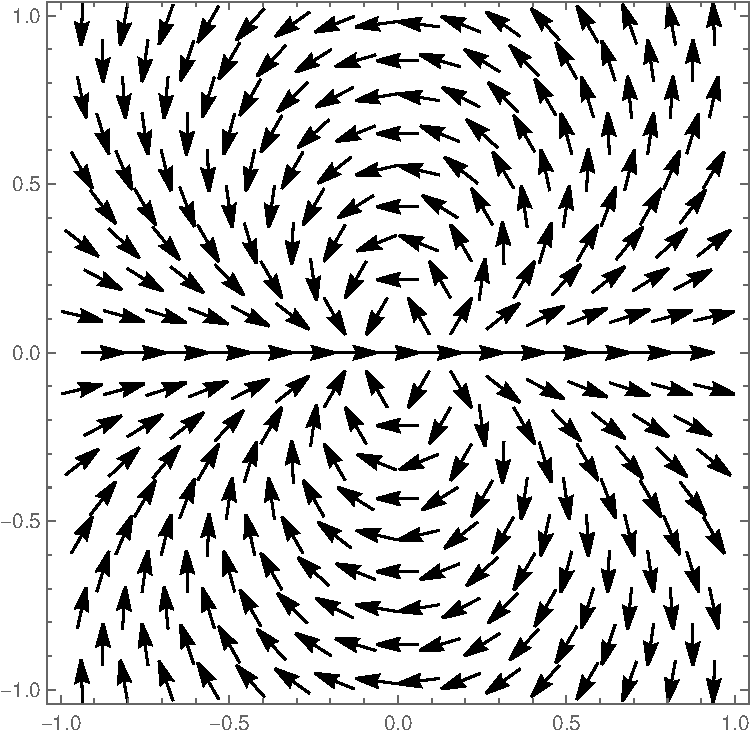
\includegraphics[scale=1,trim= 120 100 100 100,clip]{./figures/vortexn=2.pdf}
		\caption{$n=2$}
	\end{subfigure}
	\begin{subfigure}{0.45\textwidth}
		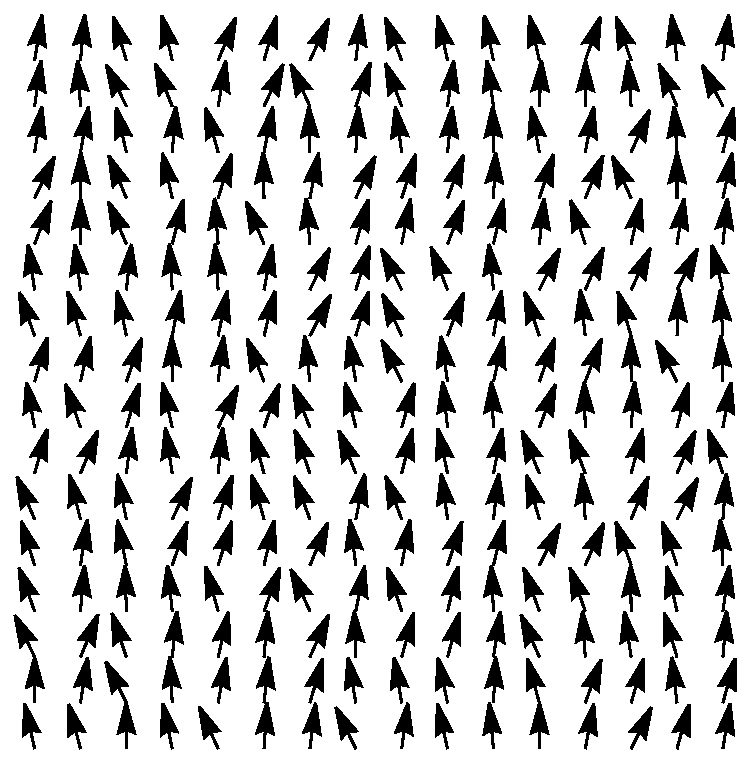
\includegraphics[scale=1,trim= 120 100 100 100,clip]{./figures/n0conf2.pdf}
		\caption{$n=0$}
	\end{subfigure}
	\begin{subfigure}{0.45\textwidth}
		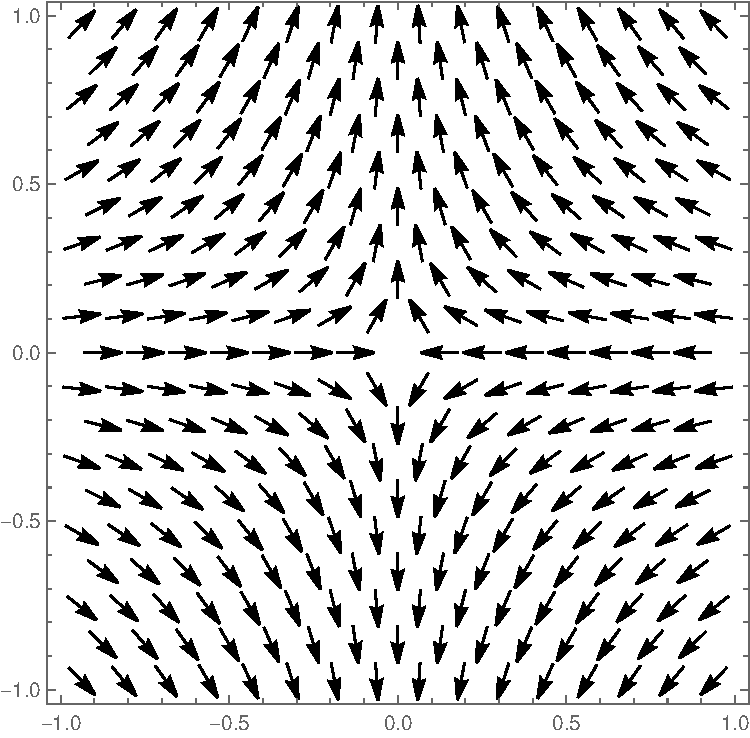
\includegraphics[scale=1,trim= 120 100 100 100,clip]{./figures/n=-1.pdf}
		\caption{$n=-1$}
	\end{subfigure}
	\begin{subfigure}{0.45\textwidth}
		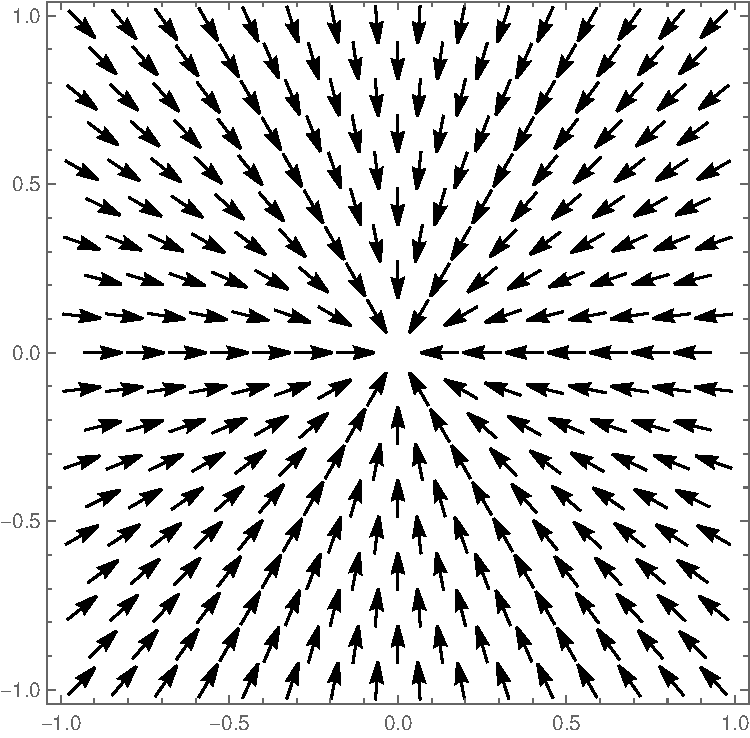
\includegraphics[scale=1,trim= 120 100 100 100,clip]{./figures/n=-1s.pdf}
		\caption{$n=1$}
	\end{subfigure}
	\caption{Configurations of spins with different winding numbers.}
	\label{fig:vortices}
\end{figure}
When we stack vortices on top of each other we can create a 1-dimensional defect called a \textit{string}, see Figure \ref{fig:string}.

\begin{figure}
	\centering
	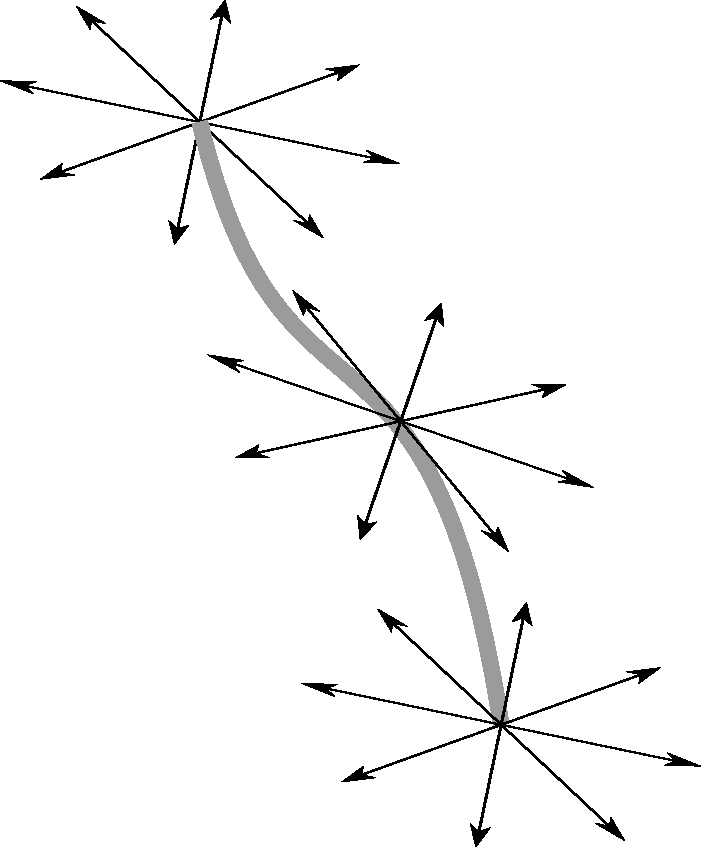
\includegraphics[scale=0.7]{./figures/string.pdf}
	\caption{Two dimensional vortices stack on top of each other in the 3-dimensional physical space forming a vortex \textit{string}.}
	\label{fig:string}
\end{figure}
%\subsection{Flux lines in type II superconductors}
\subsection{Nematics}\label{sec:nematics}
Liquid crystals are substances that share properties from both liquids and crystals. Liquid crystals possess phases such as the nematic phase, the chollesteric phase, smectic phase, etc. Nematics are liquid crystals in the nematic phase. Nematics are made of rod shaped molecules which tend to align parallel to one another. Since the orientation of the molecules does not matter, mathematically the order parameter is represented by a headless vector, $\vec{n} \equiv -\vec{n}$.


In this case, the group of symmetries of the physical 3d space is $G=\text{SO}(3)$. The group of isometries $H=D_{\infty}$ are rotations along the molecular axis and the rotations along the axis perpendicular to the molecular axis. Then, the order parameter space is $G/H = \text{SO}(3)/D_{\infty}$, which is known to be isomorphic to the real projective plane $RP^2$. The real projective plane $RP^2$ is the space formed by all lines that pass the origin in $\mathbb{R}^3$, and it is described as a half-sphere with opposite points in the equator identified. Through a direct application of the Seifert-van Kampen theorem, it can be shown that $\pi_1(RP^2) \simeq \mathbb{Z}_2$. A heuristic explanation of this fact can be described as follows: the space $RP^2$ is an hemisphere and can be flatten out to become a flat disk with the build only two types of loops, one type that is entirely inside the disk, and another one connecting two opposite points in the boundary, see Fig.\ \ref{fig:rp2}. The one inside the disk is a trivial loop since it can be reduce to a point, because $RP^2$ is simply connected within the disk. However, the one that connects opposite points in the boundary cannot be reduce to a point since the points in the boundary are fixed and cannot move. Only this class of non-trivial loop exists, so we conclude that $\pi_1(RP^2)\simeq \mathbb{Z}_2$. In conclusion, nematics enable one type of vortices. 

\begin{figure}
\centering
	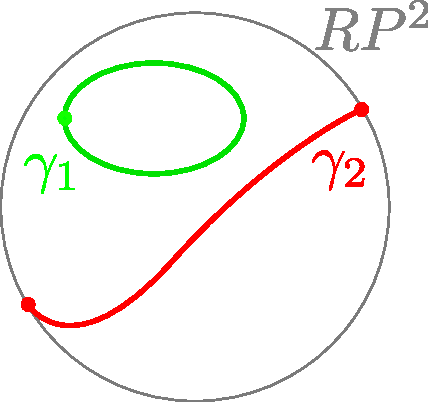
\includegraphics[scale=0.7]{./figures/rp2.pdf}
	\caption{The projective plane $RP^2$ and two types of loops $\gamma_1$ and $\gamma_2$. The loop $\gamma_1$ is a trivial loop and can be contracted to a point. However, $\gamma_2$ is a loop that connects two opposite points on the boundary, and it is the only type of loops which cannot be contracted to a point.}
	\label{fig:rp2}
\end{figure}

\begin{figure}
\centering
	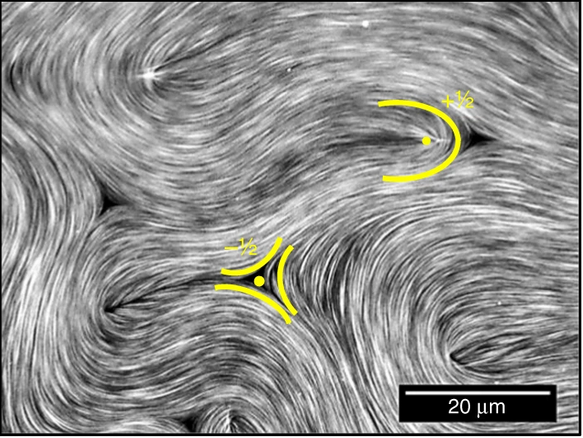
\includegraphics[scale=0.5]{./figures/vortexnematics.png}
	\caption{Vortices in a nematic represented as yellow dots with topological charges 1/2 and $-1/2$, figure taken from Ref.\ \cite{Doos2018}.}
	\label{fig:vortexnematic}
\end{figure}

However, if we constrain the molecules to live in a plane, the order parameter manifold is now a semicircle with the endpoints identified, denoted as $S^1/\mathbb{Z}_2$. The semicircle is mathematically described by $x=e^{i\varphi}$, $\varphi\in [0,\pi)$ and can be mapped to a complete circle by the function $f(x) = x^2$. Thus, the space $S^1/\mathbb{Z}_2$ is isomorphic to $S^1$. Therefore, its  first homotopy group is $\pi_1(S^1/\mathbb{Z}_2 \simeq S^1) \simeq \mathbb{Z}$. In some applications, it is convenient to take $\pi_1(S^1) \simeq \frac{1}{2}\mathbb{Z}$, since $\mathbb{Z}\simeq \frac{1}{2}\mathbb{Z}$, so the topological charge can be an integer or half-integer. In Figure \ref{fig:vortexnematic}, we see two types of vortices in a nematic with topological charges of $1/2$ and $-1/2$.

\subsection{Quantum vortices in superfluid helium}\label{sec:helium}
Helium has two isotopes, $^3$He and $^4$He, and when they become superfluids, they exhibit rotating vortex defects when stirred.

In the case of $^4$He, it becomes a superfluid only when it is cooled down below 2.17 K, and since it is a boson, its superfluid phase is related to the Bose-Einstein condensation. 

In contrast, $^3$He, the lighter helium isotope, only becomes a superfluid when its temperature drops below 0.0025 K. Since $^3$He is a fermion, its superfluid phase has a different mechanism from $^4$He. $^3$He superfluid is related to the creation of Cooper pairs (similar to superconductivity). $^3$He has two superconductivity phases and when an external magnetic field is applied to one of the phases it splits creating yet another superconducting phase.

The order parameters for $^3$He and $^4$He are their multi-particle wave functions, a complex scalar for $^4$He and a $3\times 3$ complex matrix for $^3$He. In $^4$He, we can define a Lagrangian which is symmetric under $\text{U}(1)$ that is related to global phase transformations of the wave function. However, this $\text{U}(1)$ can break since in a state like a superfluid there exists a non zero superfluid condensate. This condensate has a definite phase, so it breaks the $\text{U}(1)$ symmetry down to $I$. %its wave function satisfies the Schrödinger equation, and it is known to possess a U$(1)$ symmetry, 
 So $\pi_1(\text{U}(1)/I\simeq S^1) \simeq \mathbb{Z}$, therefore $^4$He has vortices. In fact, these vortices have their circulation quantized, so they are called quantum vortices. In order to see this, let us consider a system with $N$ bosonic particles. The wave function of $^4$He superfluid takes the form
\begin{equation}
	\psi = A e^{i\varphi(\vec{r}_1,\vec{r}_2,\dots,\vec{r}_N)},
\end{equation}
where $\varphi = \sum_i \vec{p}_{s,i}\cdot\vec{r}_i/\hbar$ and $\vec{p}_{s,i}= m \vec{v}_{s,i}$, where $m$ and $\vec{v}_{s,i}$ are the mass of  individual $^4$He atoms and the drift velocity, respectively. With this definition of the phase $\varphi$, it is straightforward that
\begin{equation}
	\vec{v}_s = \frac{\hbar}{m}\nabla \varphi.
\end{equation}
Since $\varphi$ is continuous, that means that the integral along a closed path surrounding the vortex core must be an integer multiple of $2\pi$,
\begin{equation}
	\oint d \varphi = 2\pi n, \ n\in\mathbb{Z},
\end{equation}
similar to what we encountered in the planar spin model. Computing the circulation of the vortex results in
\begin{equation}
	\Gamma = \oint \vec{v}_s \cdot d\vec{l} = \frac{nh}{m}.
\end{equation}

Experimentally, quantum vortices appear when the vessel containing $^4$He superfluid is rotated. At low angular velocities, the superfluid remains at rest while the vessel is rotated. At higher velocities, vortices appear and rotate. Ref.\  \cite{PhysRevLett.43.214} reported the first experimental observation of vortices in superfluid $^4$He. In Figure \ref{fig:heliumvortices} we see vortices formed in superfluid $^4$He droplets from numerical simulations, image taken from Ref.\ \cite{ancio2015}.

\begin{figure}
	\centering
	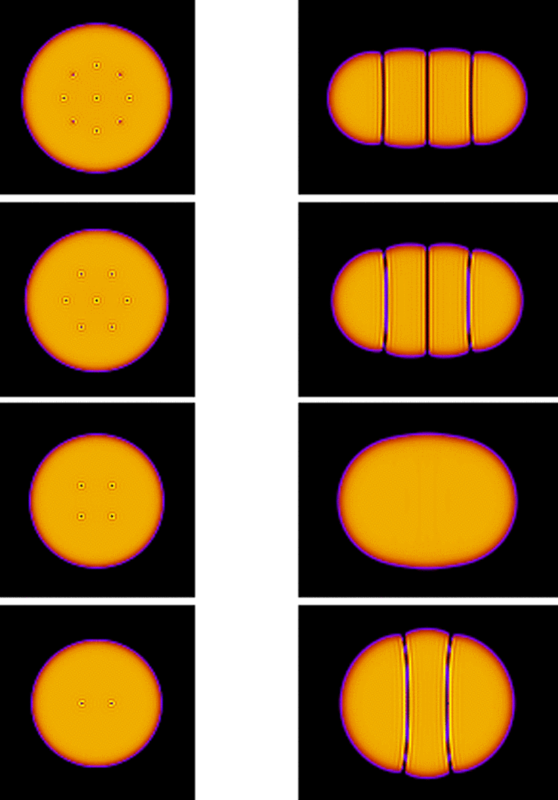
\includegraphics[scale=0.5]{./figures/hevortices.png}
	\caption{Quantum vortices in superfluid $^4$He droplets, generated by numerical simulations. We see from top to bottom, 9, 7, 4 and 2 vortices. Left panel: top view parallel to the angular momentum, $z=0$. Right panel: side view perpendicular to the angular momentum,  $x=0$. Image taken from Ref.\ \cite{ancio2015}} %The container with the superfluid is rotated, and vortices appear when there a certain threshold in the velocity is attained.}
	\label{fig:heliumvortices}
\end{figure} 


\section{Quantum field theory}\label{sec:qft}

\subsection{The vacuum as the order parameter manifold}\label{sec:vacuum}
Let us consider a theory with a scalar field $\phi$, which transforms under a representation of a Lie group of transformations $G$. Let the potential $V = V(\phi)$ be a function of the fields invariant under transformations of $G$.

If the potential  $V$ acquires a non-zero vacuum expectation value (VEV) $\phi_0$, then the symmetry group $G$ will be spontaneously broken, so $\phi$ develops a set $\mathcal{M}$ of degenerate vacua, this implies $\phi_0 \in \mathcal{M}$. All the transformations of $\phi_0$ by representations of $G$ will be genuine VEVs of the scalar field, that is, $D(g)\phi_0 \in \mathcal{M}$. Some of these transformations may lead to the same point. We define the subgroup $H\subset G$ as the group of elements of $G$ which leave $\phi_0$ invariant, that is,
\begin{equation}
	H = \{g\in G | D(g)\phi_0 = \phi_0\}.
\end{equation}
%We wish to determine the set of all possible vacua of the field $\phi$. %This set is given by all non-trivial transformations in $G$ of $\phi_0$. 
This implies that the set of all distinct transformations of $\phi_0$ is given by the quotient group $G/H$, which means that the vacuum manifold is $\mathcal{M}=G/H$.%Let $D(g)$ be a transformation that takes $\phi_0$ to some other point $\phi_1$.
%Then all the elements that take $\phi_0$ to the same point, that is, $D(g)\phi_0 = D(g')\phi_0$ if and only if $D(g') = D(g)D(h) = D(g\cdot h)$ with $h\in H$, 

In other words, the set of values of a scalar field that minimizes the potential, in a theory where a group of symmetries $G$ breaks spontaneously down to a subgroup $H\subset G$, forms a manifold which we identify as the coset space $G/H$. This way, we can take the vacuum manifold as the order parameter manifold, and the order parameter as a state in the vacuum.

%In field theory we sometimes are interested in static solutions to the field equations with a definite energy which we call \textbf{solitons}.
%\begin{definition}
%A \textbf{soliton} as solutions to field equations with the following properties:
%\begin{enumerate}
%\item The energy density is finite and localized in space.
%\item They preserve their shape while propagating at constant speed. From this it follows that they are static in time.
%\end{enumerate}
%\end{definition}



\subsection{Vacuum topology}\label{sec:vactop}

 Let us consider a Lagrangian density of a complex scalar field $\phi(x) = \phi(t,\vec{x})\in \mathbb{C}$ as
\begin{equation}
	\mathcal{L} = \frac{1}{2}\partial^{\mu} \phi^* \partial_{\mu} \phi  - V(\phi).
\end{equation}
Then its energy density is
\begin{equation}
		\epsilon = \frac{1}{2}|\partial_t \phi|^2 + \frac{1}{2}|\nabla \phi|^2 + V(\phi).
\end{equation}
For the total energy of the derivative terms to be finite, we require that
\begin{equation}
	\lim_{|\vec{x}|\to\infty} \phi(x) \in \mathcal{M},
\end{equation}
which means that at spatial infinity the field configuration $\phi$ takes a value in the vacuum manifold $\mathcal{M}$. The value of the field can be different in different directions at spatial infinity. Therefore, a field configuration defines a map from $S^{d-1}_{\infty}$, the $(d-1)$-sphere at the spatial infinity in $\mathbb{R}^d$, to the vacuum manifold $\mathcal{M}$
\begin{equation}
	\phi^{\infty} : S^{d-1}_{\infty}\to\mathcal{M},
\end{equation}
which means that the map $\phi^{\infty}$ defines a $(d-1)$-loop in $\mathcal{M}$.
As we saw earlier, two field configurations $\phi$ and $\phi'$ are homotopic, or topologically equivalent, if their field configurations at infinity $\phi^{\infty}$ and $\phi'^{\infty}$ can be deformed continuously into one another, that is, if they fall into the same equivalence class. This suggests that the topological information of the field configurations is com\-plete\-ly defined by the homotopy group of the vacuum manifold $\pi_{d-1}(\mathcal{M})$.

%It is known that in a linear field theory (linear in the equations of motion), two field configurations are homotopic if they have the same asymptotic behavior. However, two field configurations $\phi$, $\phi'$ can still be homotopic even if their asymptotic values $\phi^{\infty}$ and $\phi'^{\infty}$ are different, as long as these two are homotopic. This implies that the topological information of the field configuration is completely defined by the homotopy class of the map $\phi^{\infty}$ which is an element of $\pi_{d-1}(\mathcal{M})$.

\subsection{The Kibble mechanism}\label{sec:kibble}

 Several phase transitions took place in the early universe due to the cooling down of the universe as a consequence of its expansion. The fast expansion, at the late stages of inflation, produced casually uncorrelated regions because the correlation length $\sim H^{-1}$ was shorter than the size of the universe, where $H$ is Hubble's parameter. These regions, in principle, could have different configurations of vacuum states for some field. At some instant, the correlation length grew faster than the expansion rate of the universe, so the regions grew and became casually connected. In the interfaces between these regions, topological defects could form. The mechanism of having topological defects due to phase transitions in the early universe is known as the \textit{Kibble mechanism} \cite{Kibble1976,Kibble1980}. 
 
 %An example of the Kibble mechanism is the one that produces \textit{cosmic strings}. 


\section{The Standard Model}\label{sec:SM}
In the Standard Model of particle physics, particles are classified as either fermions or bosons, where fermions are particles with half-integer spin and bosons with an integer spin. 

A refined classification of fermions distinguishes between leptons and quarks, where only the quarks posses color charge. Also, fermions in general have left- or right-handed chirality. For massless fermions they are in\-de\-pend\-ent of each other. 

 Leptons possess a quantum number called the \textit{lepton number} $L$. Each particle in the lepton family is assigned a lepton number of $L=1$. Similarly, quarks posses a \textit{baryon number} $B$, and each quark is given a baryon number of $B=1/3$. Moreover, we assign $L=-1$ and $B=-1/3$ to the anti-leptons and anti-quarks, respectively. In nature, only combinations of quarks that give an integer baryon number are realized; they are called hadrons. 

Bosons with a spin 1 in the Standard Model are called the force carriers, such as the photon that is the electromagnetic force carrier, the gluons that mediate the strong interaction and the $W^{\pm}$, $Z$ bosons which mediate the weak interaction. Finally, the Higgs boson is the only elementary scalar particle, with spin 0. Along with Yukawa couplings, it is responsible of giving mass to other elementary particles.

There are two kinds of symmetries in physics: global symmetries and local or gauge symmetries. Normally, global symmetries are approximate, they arise from a hierarchy of energy scales and are manifest in the form of multiplets of particles. For example, in QCD with massless quarks the only dimensionful quantity is $\Lambda_{\text{QCD}}\sim 300$ MeV and since the masses of the up and down quarks are far below this energy scale, there is an approximative SU$(2)$ symmetry known as the isospin  symmetry. On the other hand, gauge symmetries are redundancies in the formulation and are impossible to break. However, there is no fundamental reason for a global symmetry not to break. There are exceptions to the rule, one of them is Lorentz global symmetry that is related to CPT invariance. 
In the Standard Model of  particle physics, there is another exact global symmetry: the difference between the baryon and lepton number is conserved. 

\subsection{The global U$(1)_{B-L}$ symmetry}\label{sec:globalU} 
It is known that by Noether's theorem, both lepton and baryon vector currents are conserved classically. For leptons and quarks, their corresponding currents read
%(with Dirac neutrinos)
\begin{eqnarray}
	j_L^{\mu} & = & \sum_{f\in\text{lepton}} \left[\bar{f}_L \gamma^{\mu}f_L+\bar{f}_R \gamma^{\mu}f_R \right]\nonumber\\
	j_B^{\mu} & = & \sum_{q\in\text{quarks}} \left[\bar{q}_L \gamma^{\mu}q_L+\bar{q}_R \gamma^{\mu}q_R \right].
\end{eqnarray}
As we mentioned, at the classical level these currents are conserved,
\begin{eqnarray}
	\partial^{\mu}j_{\mu}^L & = & 0\nonumber\\
	\partial^{\mu}j_{\mu}^B & = & 0,
\end{eqnarray}
which implies both lepton and baryon number conservation. Upon quantiza\-tion, we do not expect any anomalies in these vector currents. We only expect an anomaly in the axial current,
\begin{equation}
	j^{\mu}_5  =  \sum_{f\in\text{lepton}} \left[\bar{f}_L \gamma^5\gamma^{\mu}f_L+\bar{f}_R \gamma^5\gamma^{\mu}f_R \right].
\end{equation}
However, this is not the complete picture, in fact, the anomaly can be moved from the axial current to the vector current through a gauge invariant regularization, as reviewed in Ref.\ \cite{10.1088/978-1-6817-4457-5}. 

In fact, upon quantization the same divergence in the vector currents in both leptonic and baryonic sector arise
\begin{eqnarray}
	\partial^{\mu}j_{\mu}^L & = &-\frac{N_g g^2}{32\pi^2}\text{Tr}[W_{\mu\nu}\tilde W^{\mu\nu}]\nonumber\\
		\partial^{\mu}j_{\mu}^{B} & = & -\frac{N_g g^2}{32\pi^2}\text{Tr}[W_{\mu\nu}\tilde W^{\mu\nu}],
\end{eqnarray}
where $W^{\mu\nu}$ is the $\text{SU}(2)_L$ field strength tensor in the Standard Model, $\tilde W^{\mu\nu} = \epsilon_{\mu\nu\rho\sigma}W^{\rho\sigma}$, $g$ is the weak gauge coupling and $N_g$ is the number of fermion generations.

Theoretically, these anomalous currents allow for the baryon or lepton number violation; however, no process that realizes such violation has ever been observed experimentally. If violations of the baryon number exist, there are several ways that a proton can decay while preserving the laws of energy conservation, angular momentum conservation, and electric charge con\-ser\-va\-tion. We list some examples of proton channel decays \cite{Primakoff1981}
\begin{gather} 
 p \to e^+ \bar{\nu}_e{\nu}_e, \ \ \ p \to  e^+e^+  e^- ,\ \ \ p \to  e^+\mu^+  \mu^-,\nonumber \\
 p \to e^+ \gamma,\ \ \ p \to \mu^+\gamma, \nonumber\\
 p  \to  e^+ \pi^0,\ \ \ p  \to  \bar{\nu}_e\pi^+, \ \ \ p  \to  \mu^+ K^0, \ \ \ p  \to  \bar{\nu}_{\mu}K^+.
\end{gather}
In all these processes, the charge $B-L=1$ is conserved, where $B\in\{1,0\}$ and $L\in\{0,-1\}$. In order to explain the conservation of the $B-L$ charge theoretically, we define a new current $j_{\mu}^{B-L}=j_{\mu}^B-j_{\mu}^L$, which satisfies
\begin{equation}
	\partial^{\mu}(j_{\mu}^{B-L}) = 0.
\end{equation}
This implies the conservation of the $B-L$ charge.
Conservation of the $B-L$ charge is associated with a global U$(1)$ symmetry, which we call U$(1)_{B-L}$.% We wonder if possibly a particle could mediate processes that conserve $B-L$ charge. 